\documentclass[a4paper, 12pt]{article}
\usepackage{listings} 
\usepackage{xcolor}
\usepackage{mdframed}
\usepackage{graphicx}
\usepackage{pgfplots}

% Allows for floating images
\usepackage{float}
\usepackage{mathtools}

% Custom 1 inch margins
\usepackage[margin=1.00in]{geometry}

% Custom Floor and Ceiling operators
\DeclarePairedDelimiter\ceil{\lceil}{\rceil}
\DeclarePairedDelimiter\floor{\lfloor}{\rfloor}

% Custom background color for code listings
\definecolor{code-gray}{gray}{0.93}

% Beginning of document
\begin{document}
\title{ECE 443 - Homework \#3}
\author{Collin Heist}
\date{\today}
\maketitle
\pagenumbering{arabic}

\section{Findings}
According to the Tracealyzer program, the Idle task takes up about 0.843\% of the CPU. This is about what I expected, especially for a program that switches to the idle task so frequently; although in a larger program I suspect this should be much smaller.

I suspect that the reason Task 2 takes up slightly (0.5\%) more CPU usage is entirely related to where I stopped the program. However, I am not sure about this.

\section{Results}
Below is a screen capture of the Actor Statistics Report. As expected, the percent of the time that the CPU spends on the non-idle tasks is significantly higher than that of the idle task.

\begin{figure}[H]
\centering
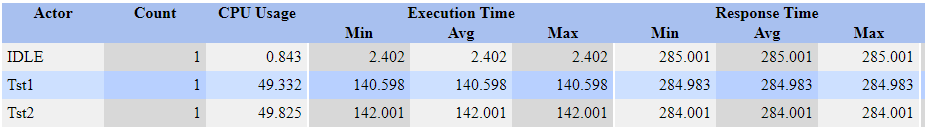
\includegraphics[width=\textwidth]{pic.png}
\caption{Actor Statistics Report}
\label{fig:img00}
\end{figure}

\end{document}